
 
\subsection{Visualizing the convolution kernels} \label{sec:visualize_operator}
%
\begin{figure}[t] \label{fig:mixing_kernel}
\centering
%\captionsetup[subfigure]{labelformat=empty}
\subfigure{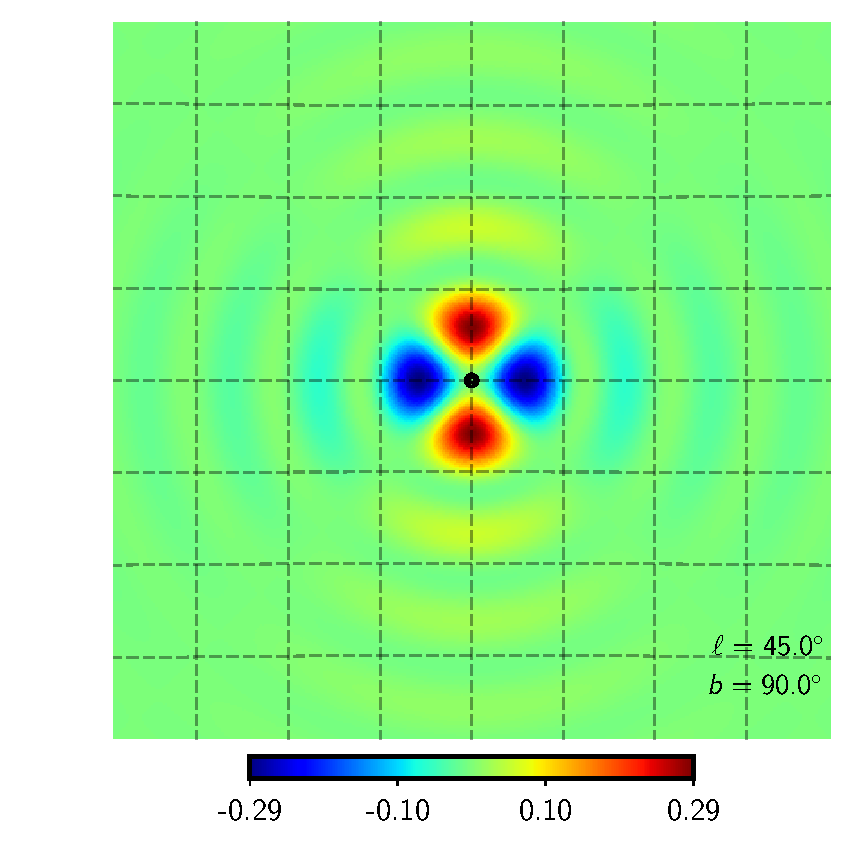
\includegraphics[width=0.16\columnwidth]{kernel/qu2eb_ker_r_lat90_lon45.pdf}}\hspace{-2mm}
\subfigure{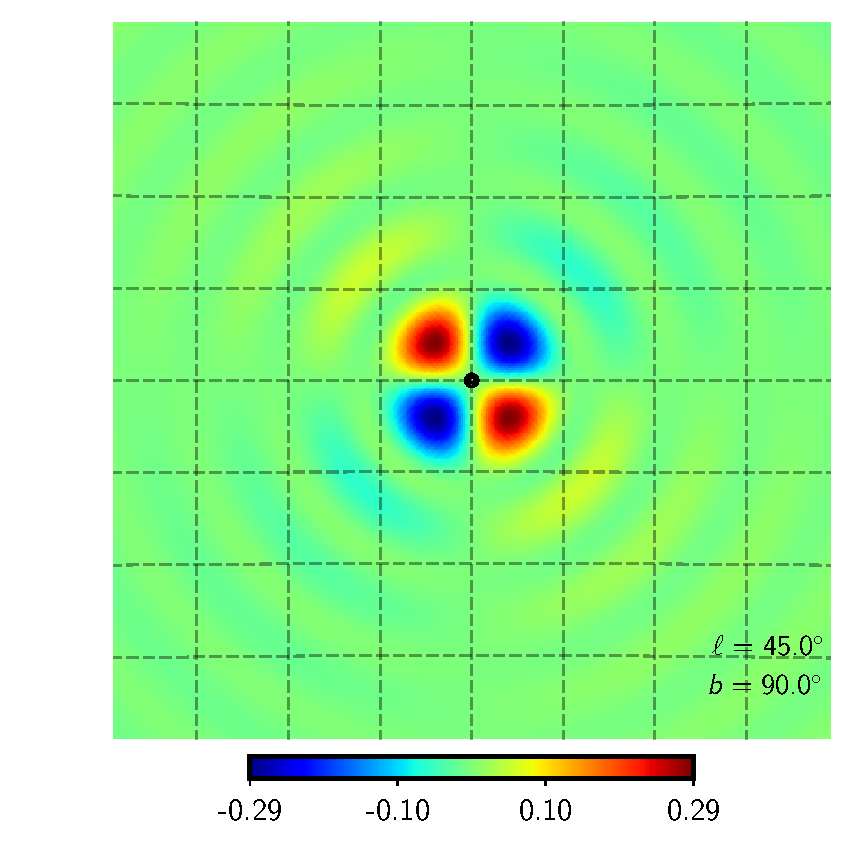
\includegraphics[width=0.16\columnwidth]{kernel/qu2eb_ker_i_lat90_lon45.pdf}}\hspace{-2mm}
\subfigure{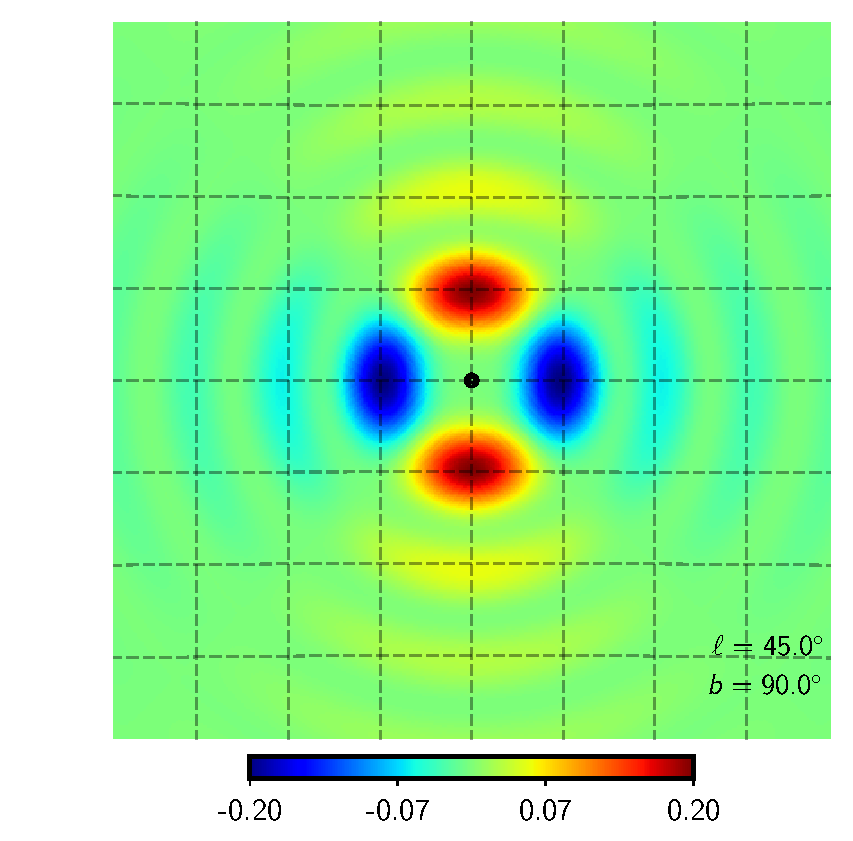
\includegraphics[width=0.16\columnwidth]{kernel/qu2ebqu_ker_r_lat90_lon45.pdf}}\hspace{-2mm}
\subfigure{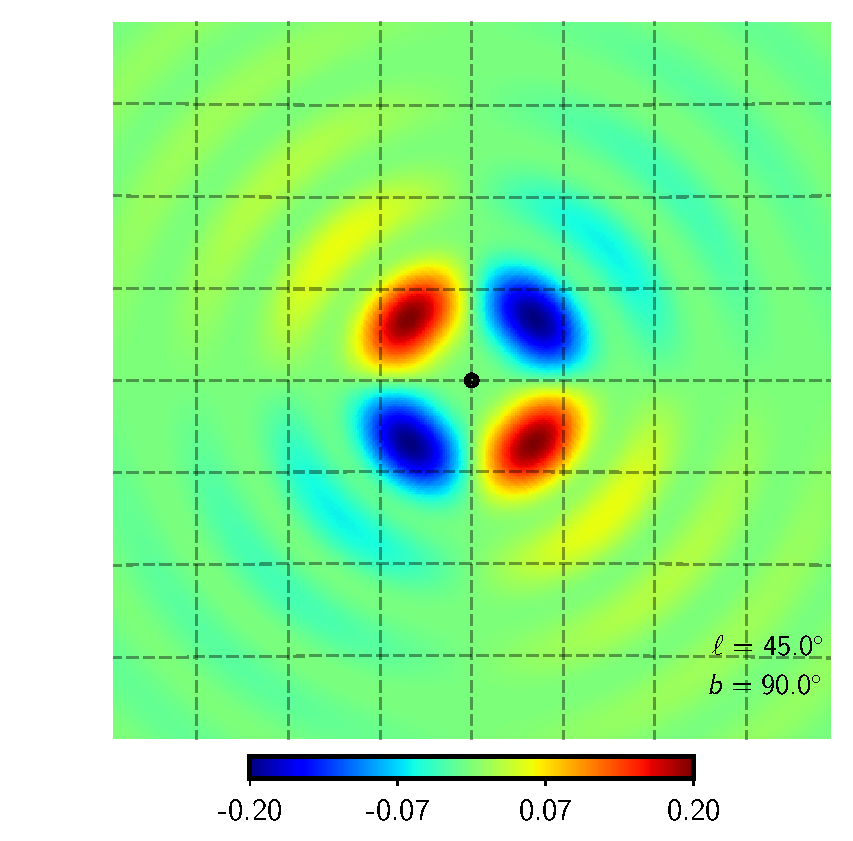
\includegraphics[width=0.16\columnwidth]{kernel/qu2ebqu_ker_i_lat90_lon45.pdf}}\hspace{-2mm}
\subfigure{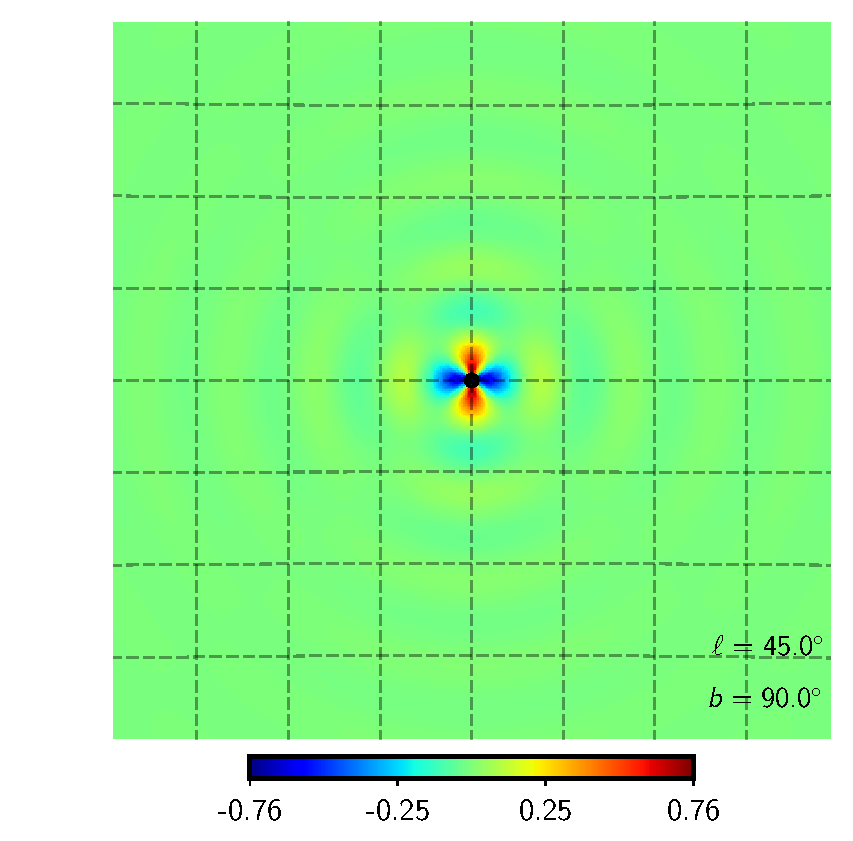
\includegraphics[width=0.16\columnwidth]{kernel/I_ker_r_lat90_lon45.pdf}}\hspace{-2mm}
\subfigure{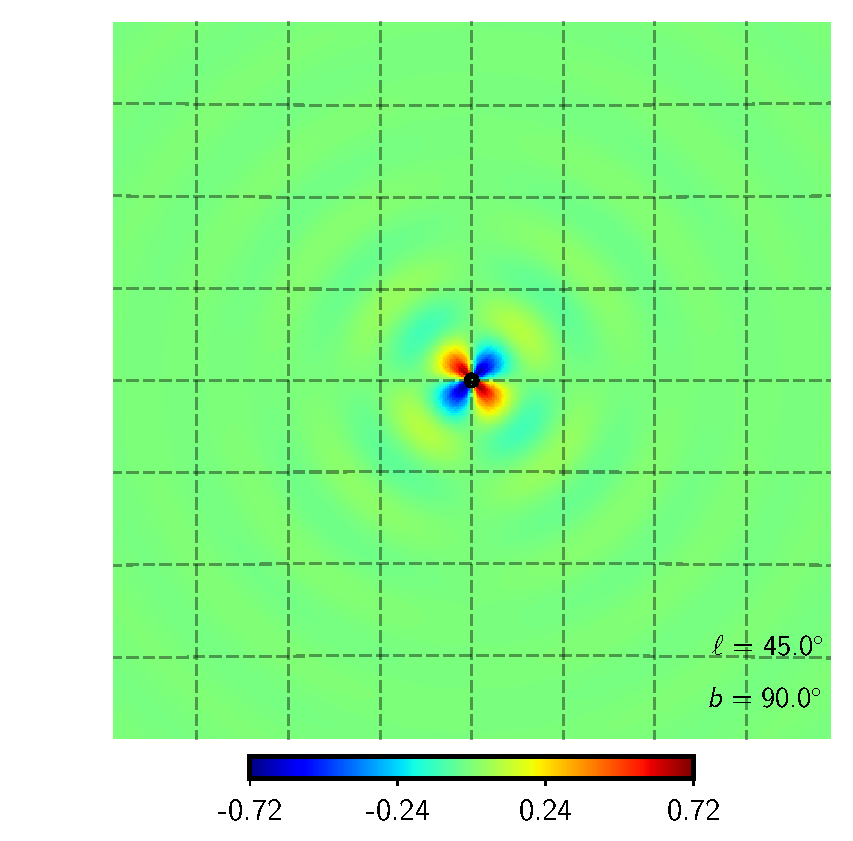
\includegraphics[width=0.16\columnwidth]{kernel/I_ker_i_lat90_lon45.pdf}}\\[-2ex]
\subfigure{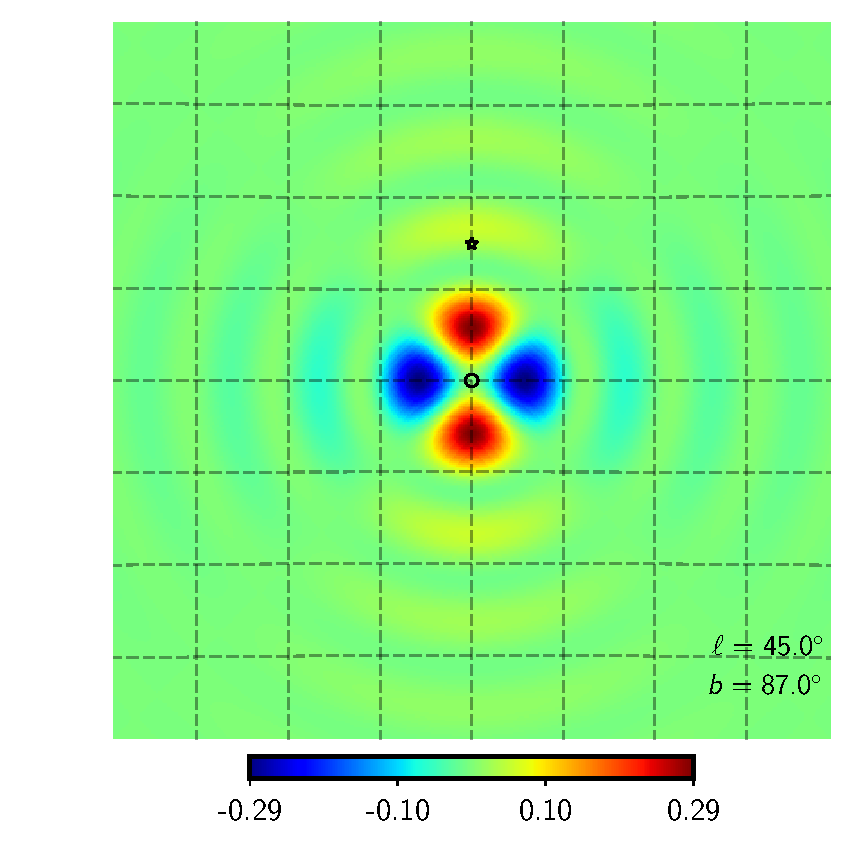
\includegraphics[width=0.16\columnwidth]{kernel/qu2eb_ker_r_lat87_lon45.pdf}}\hspace{-2mm}
\subfigure{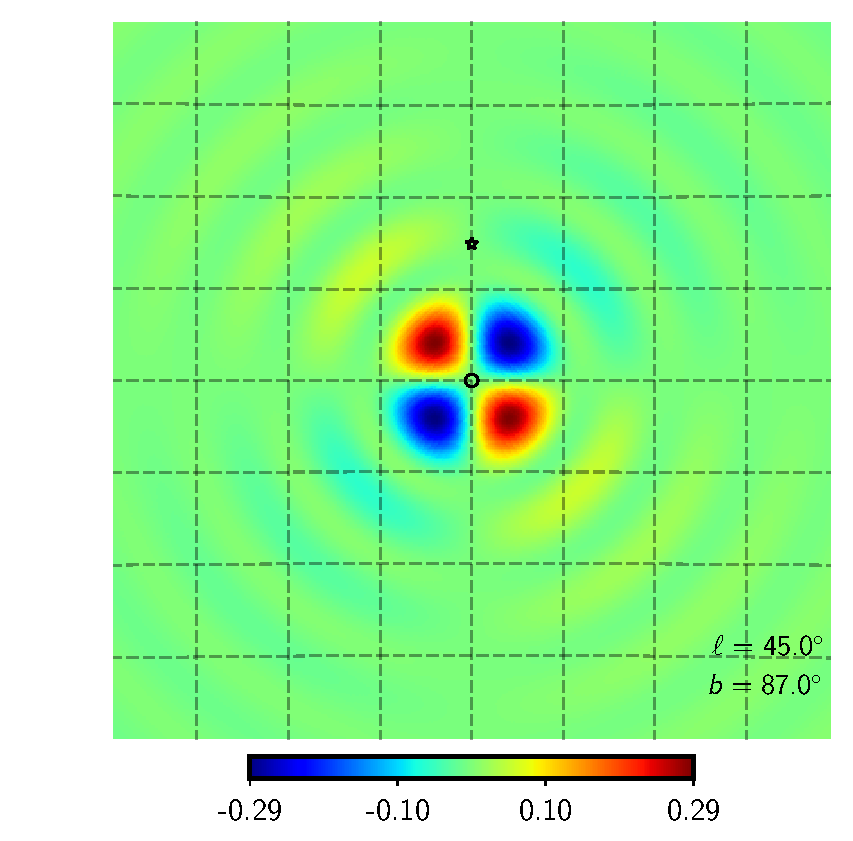
\includegraphics[width=0.16\columnwidth]{kernel/qu2eb_ker_i_lat87_lon45.pdf}}\hspace{-2mm}
\subfigure{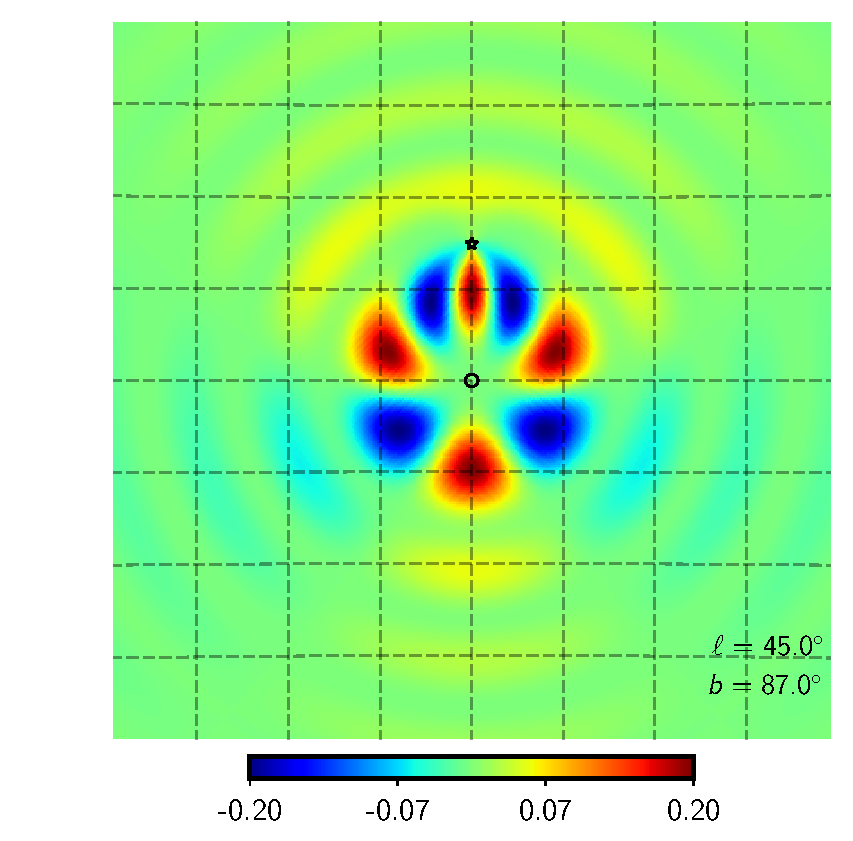
\includegraphics[width=0.16\columnwidth]{kernel/qu2ebqu_ker_r_lat87_lon45.pdf}}\hspace{-2mm}
\subfigure{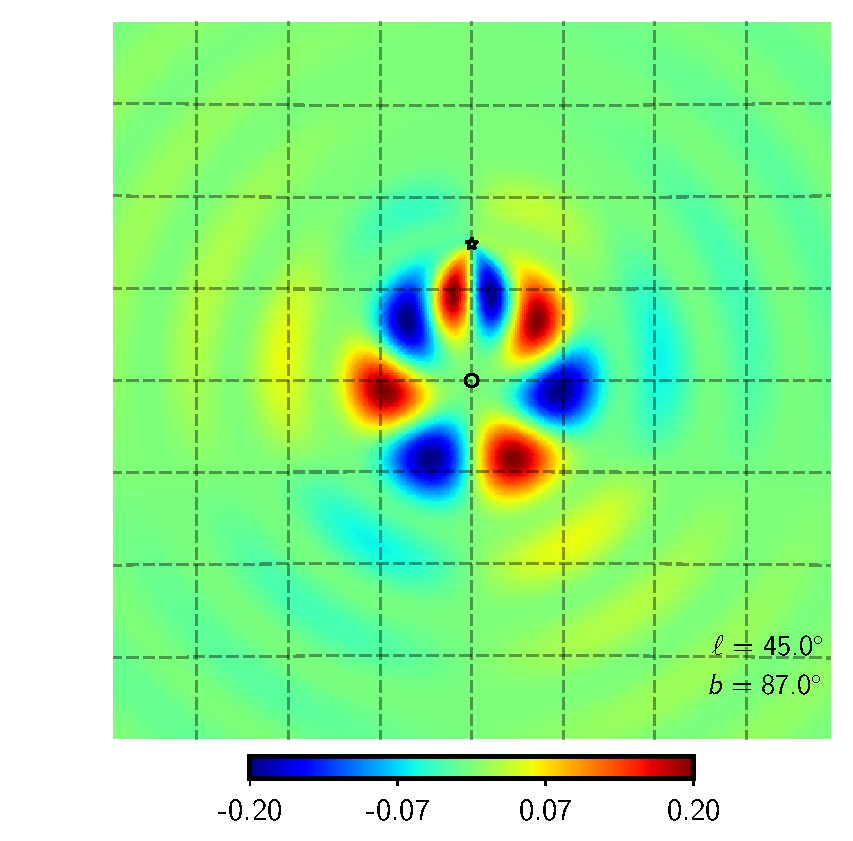
\includegraphics[width=0.16\columnwidth]{kernel/qu2ebqu_ker_i_lat87_lon45.pdf}}\hspace{-2mm}
\subfigure{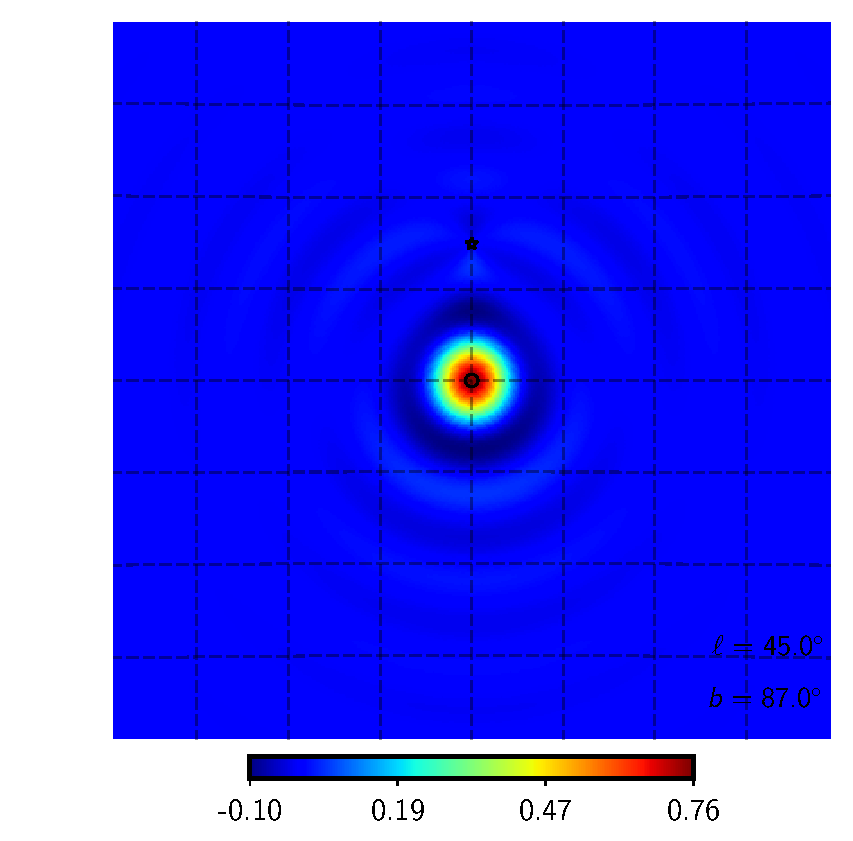
\includegraphics[width=0.16\columnwidth]{kernel/I_ker_r_lat87_lon45.pdf}}\hspace{-2mm}
\subfigure{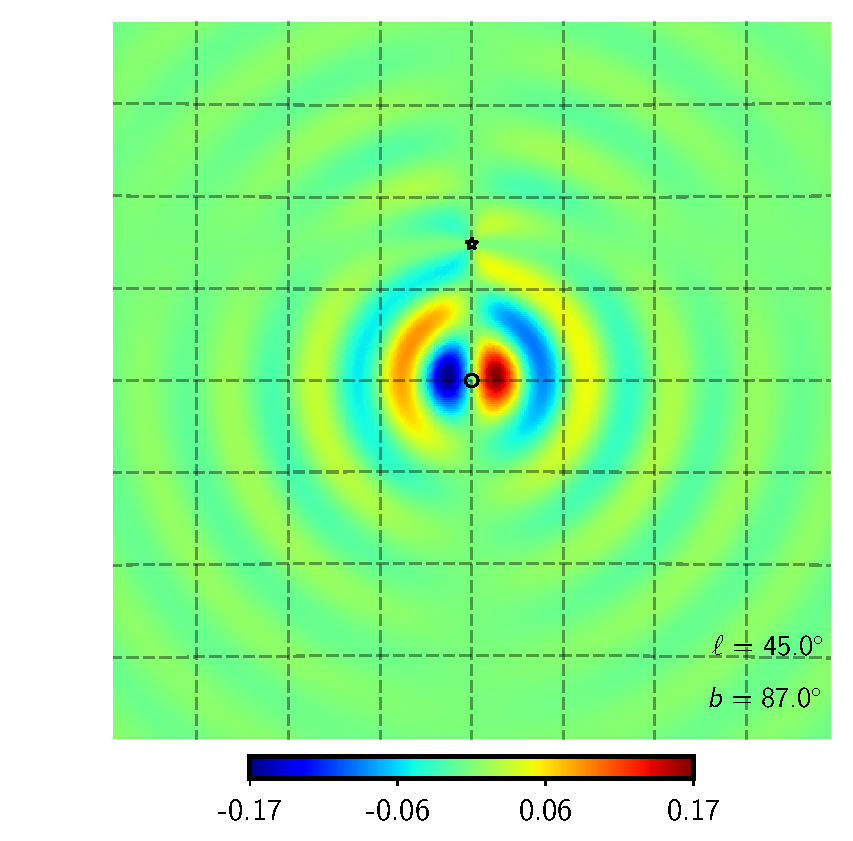
\includegraphics[width=0.16\columnwidth]{kernel/I_ker_i_lat87_lon45.pdf}}\\[-2ex]
%\subfigure{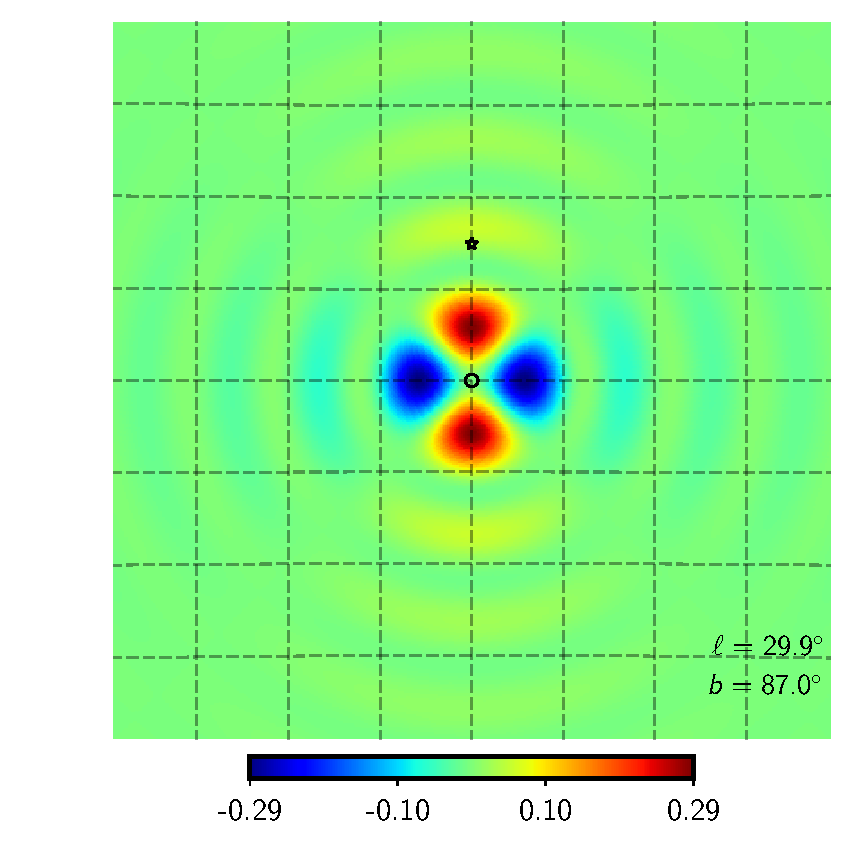
\includegraphics[width=0.16\columnwidth]{kernel/qu2eb_ker_r_lat87_lon30.pdf}}\hspace{-2mm}
%\subfigure{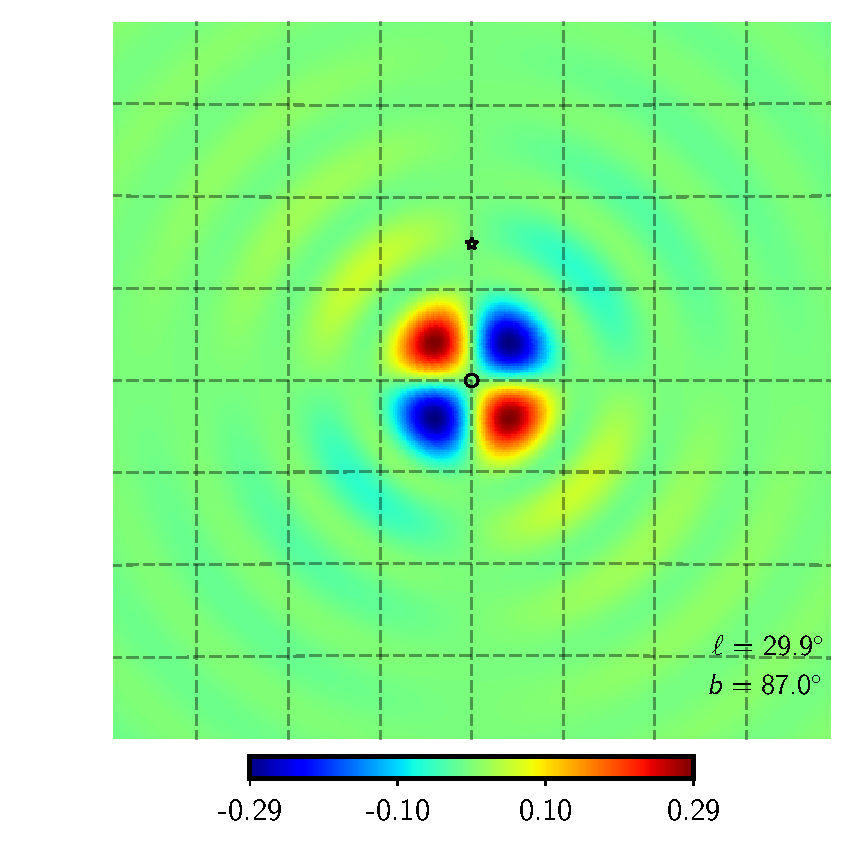
\includegraphics[width=0.16\columnwidth]{kernel/qu2eb_ker_i_lat87_lon30.pdf}}\hspace{-2mm}
%\subfigure{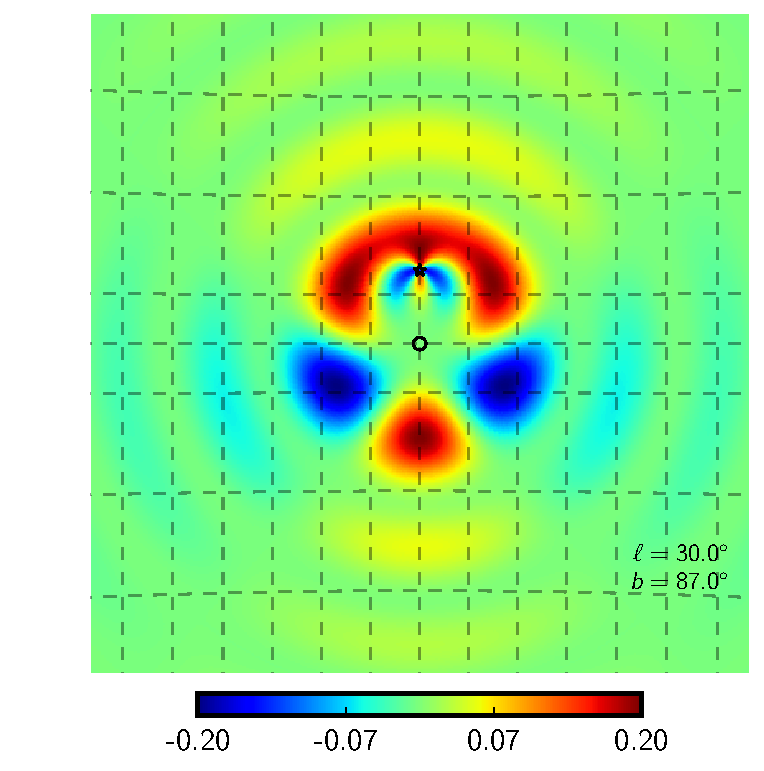
\includegraphics[width=0.16\columnwidth]{kernel/qu2ebqu_ker_r_lat87_lon30.pdf}}\hspace{-2mm}
%\subfigure{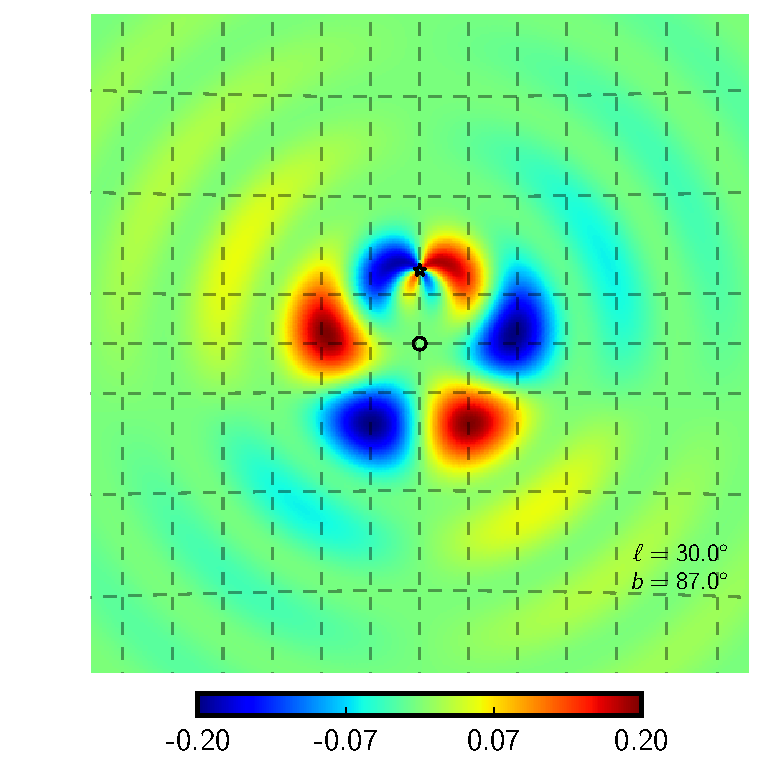
\includegraphics[width=0.16\columnwidth]{kernel/qu2ebqu_ker_i_lat87_lon30.pdf}}\hspace{-2mm}
%\subfigure{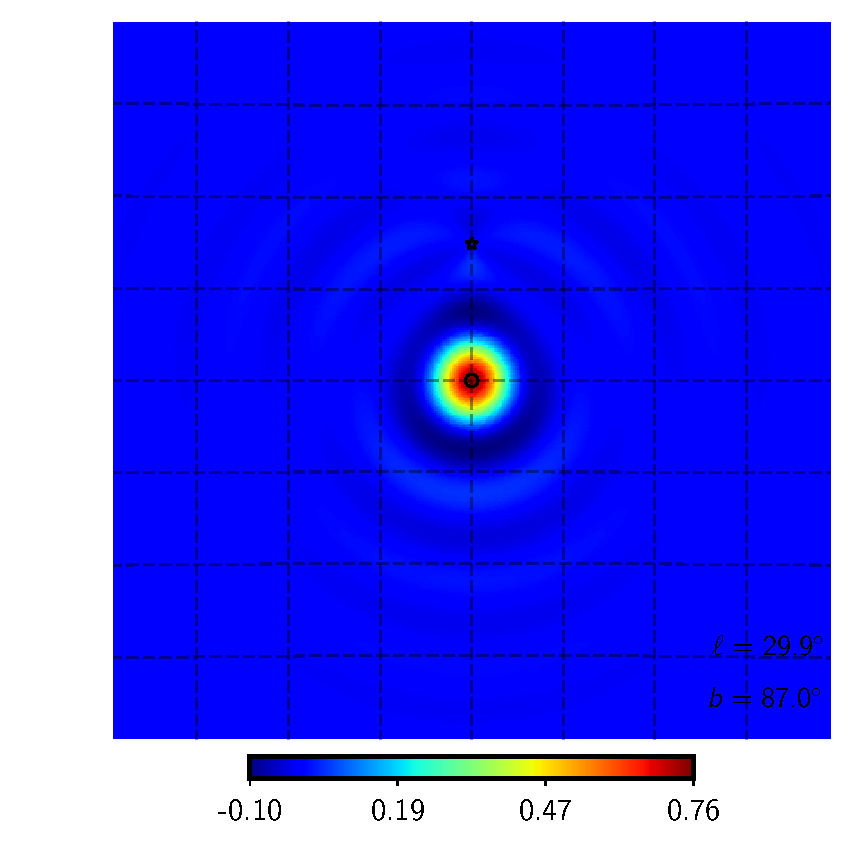
\includegraphics[width=0.16\columnwidth]{kernel/I_ker_r_lat87_lon30.pdf}}\hspace{-2mm}
%\subfigure{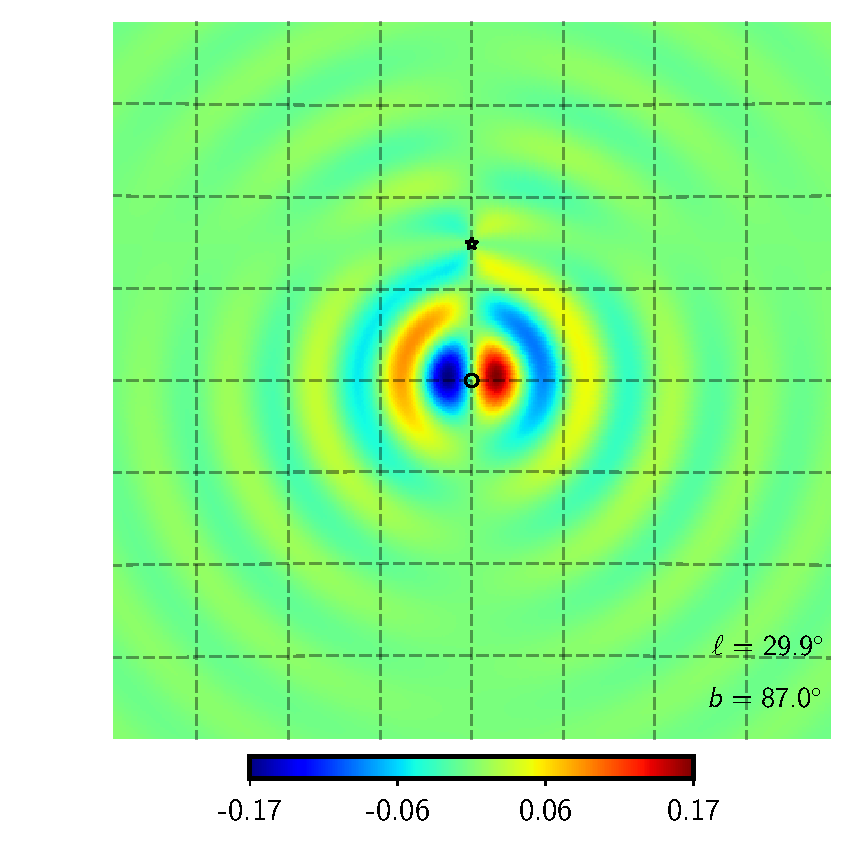
\includegraphics[width=0.16\columnwidth]{kernel/I_ker_i_lat87_lon30.pdf}}\\[-2ex]
\subfigure{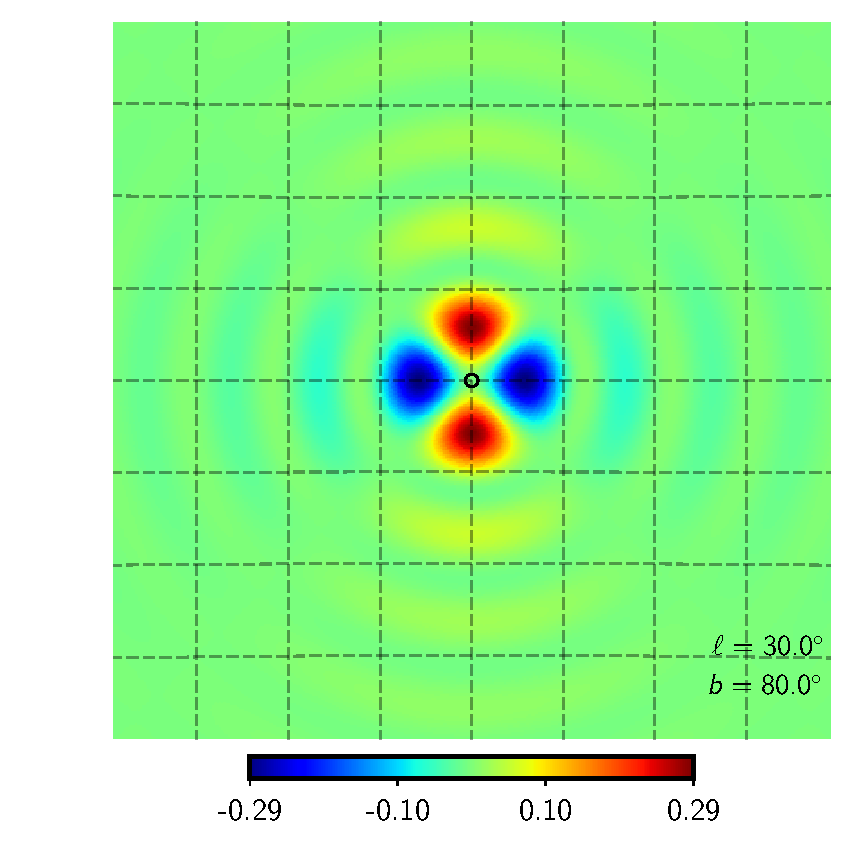
\includegraphics[width=0.16\columnwidth]{kernel/qu2eb_ker_r_lat80_lon30.pdf}}\hspace{-2mm}
\subfigure{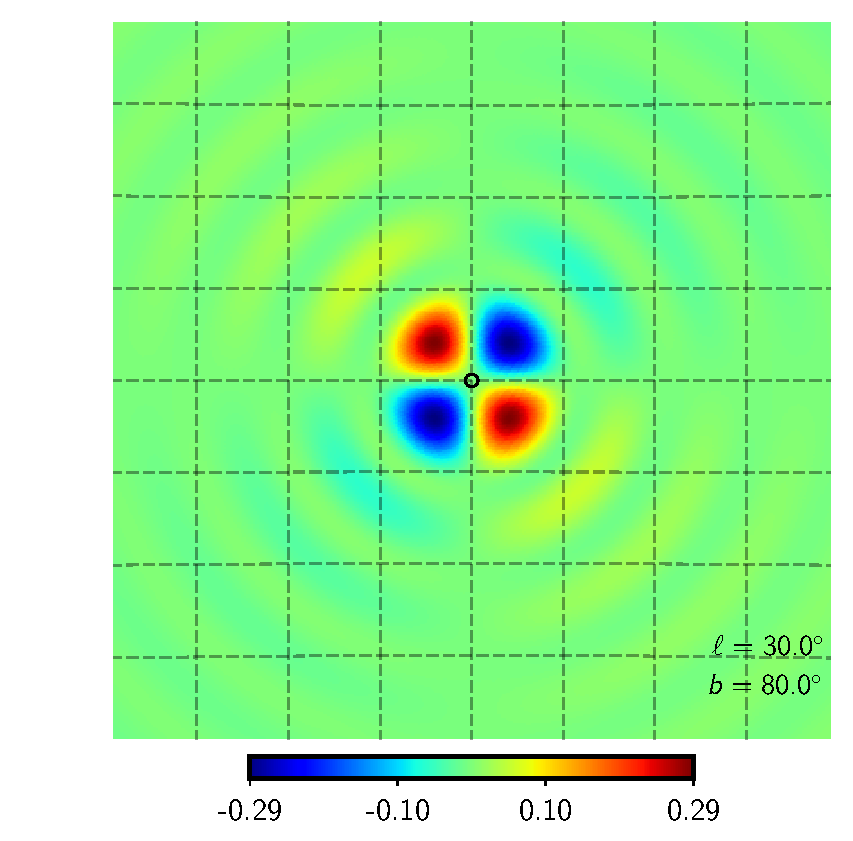
\includegraphics[width=0.16\columnwidth]{kernel/qu2eb_ker_i_lat80_lon30.pdf}}\hspace{-2mm}
\subfigure{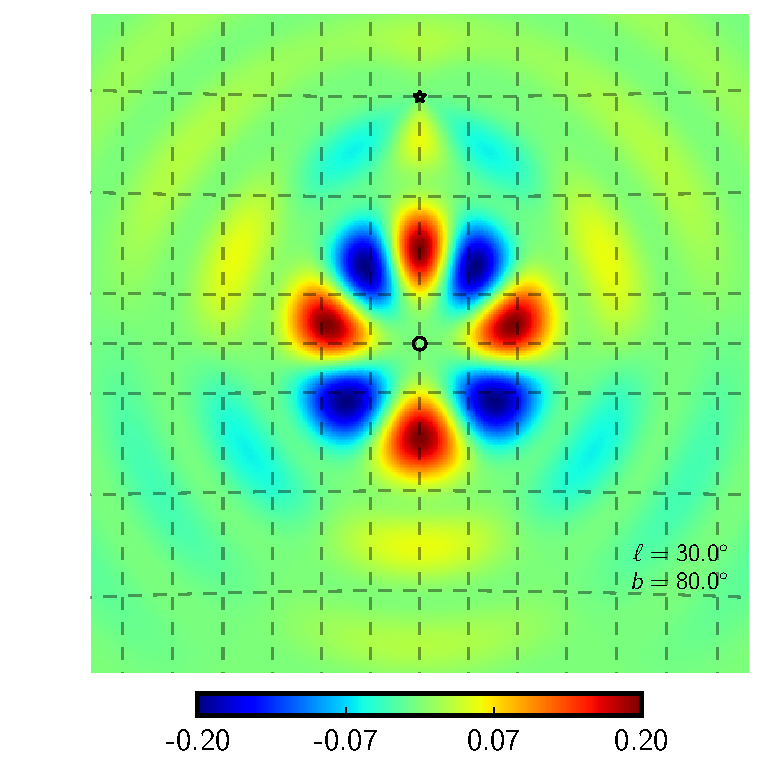
\includegraphics[width=0.16\columnwidth]{kernel/qu2ebqu_ker_r_lat80_lon30.pdf}}\hspace{-2mm}
\subfigure{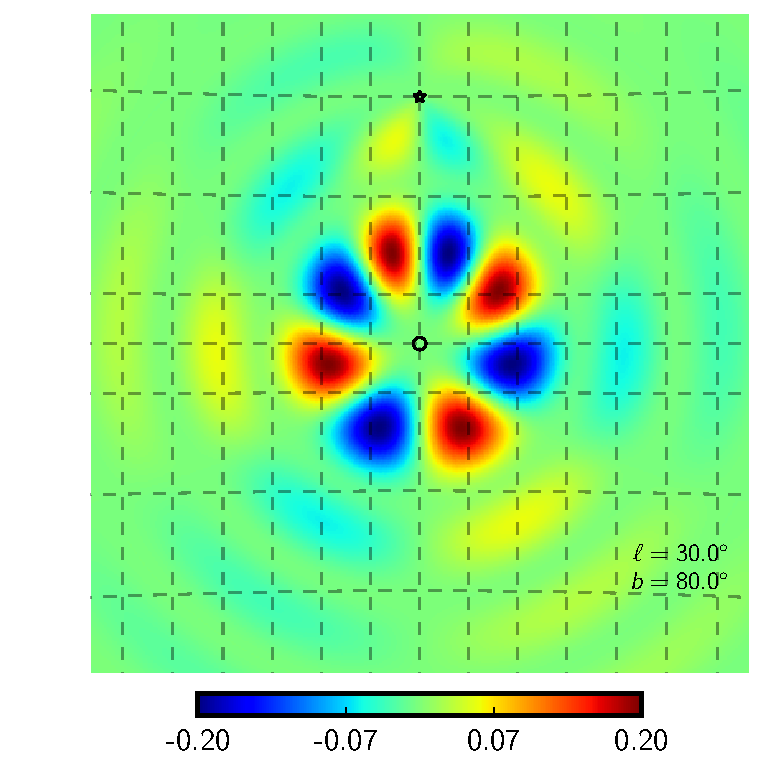
\includegraphics[width=0.16\columnwidth]{kernel/qu2ebqu_ker_i_lat80_lon30.pdf}}\hspace{-2mm}
\subfigure{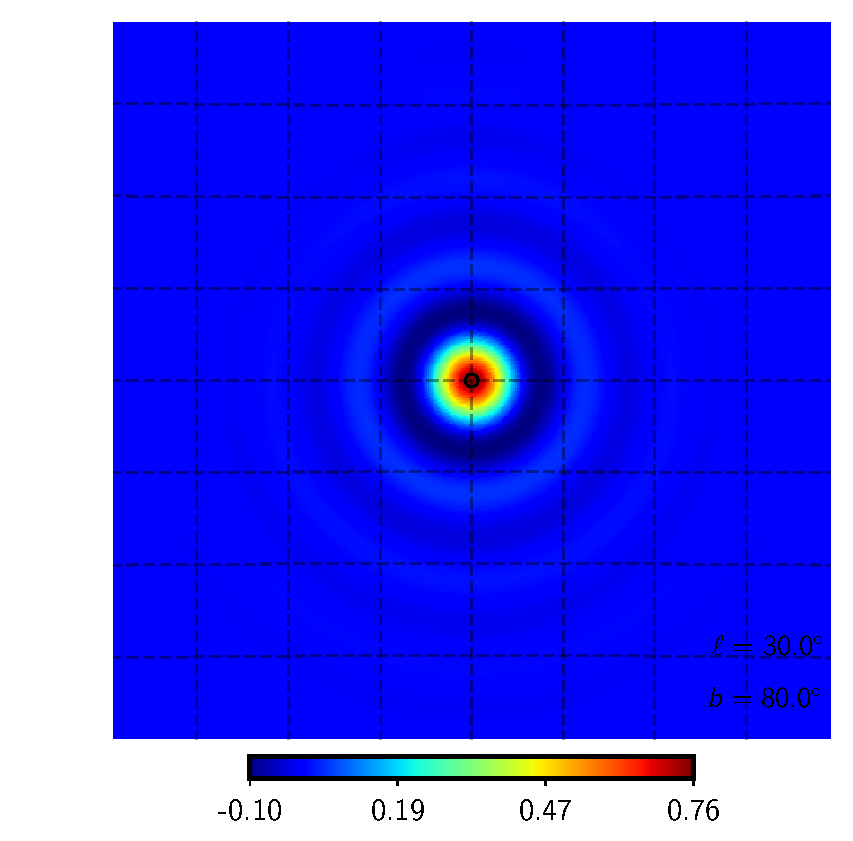
\includegraphics[width=0.16\columnwidth]{kernel/I_ker_r_lat80_lon30.pdf}}\hspace{-2mm}
\subfigure{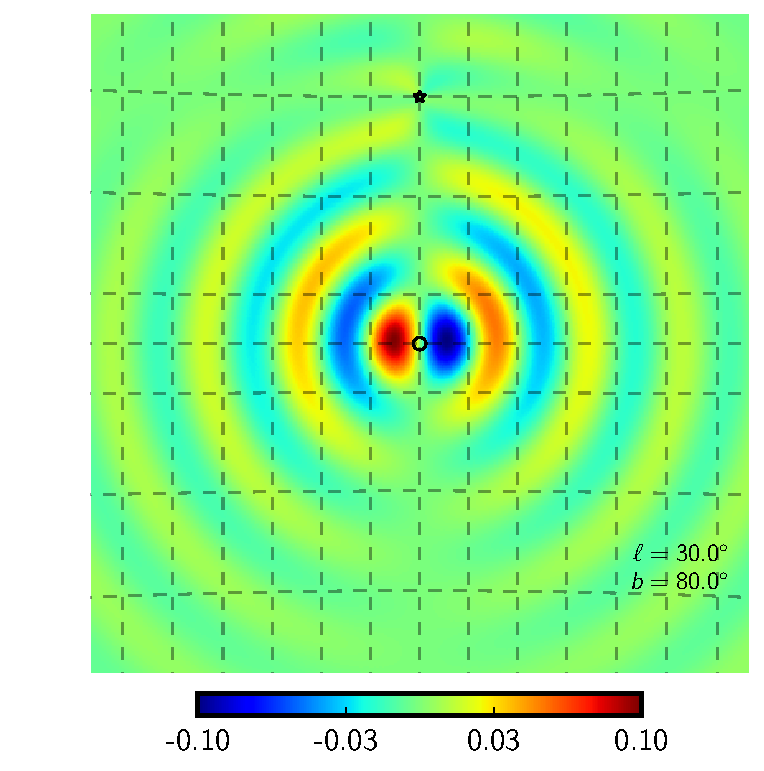
\includegraphics[width=0.16\columnwidth]{kernel/I_ker_i_lat80_lon30.pdf}}\\[-2ex]
\subfigure[$\mathcal{M}_r$]{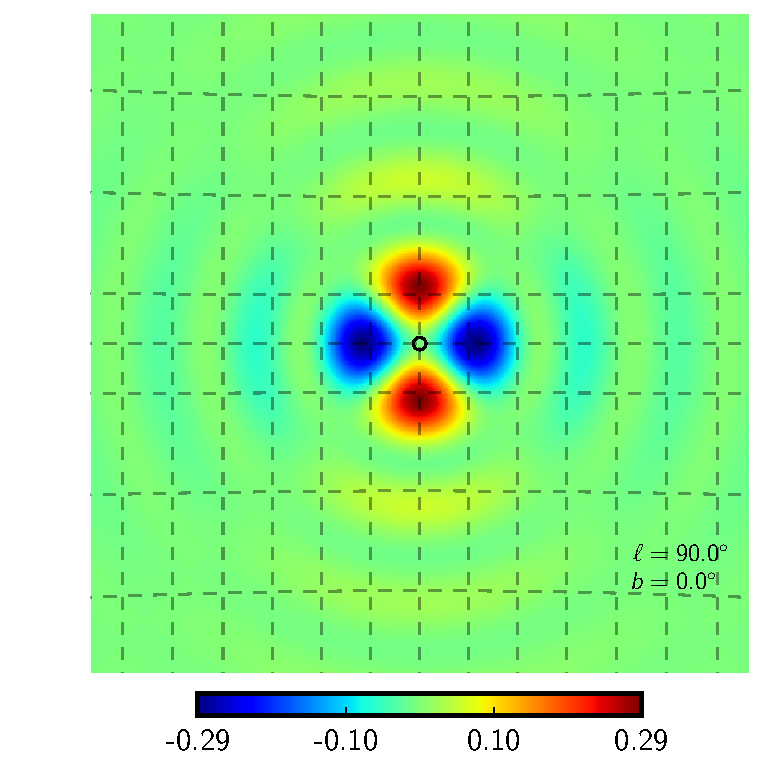
\includegraphics[width=0.16\columnwidth]{kernel/qu2eb_ker_r_lat0_lon90.pdf}}\hspace{-2mm}
\subfigure[$\mathcal{M}_i$]{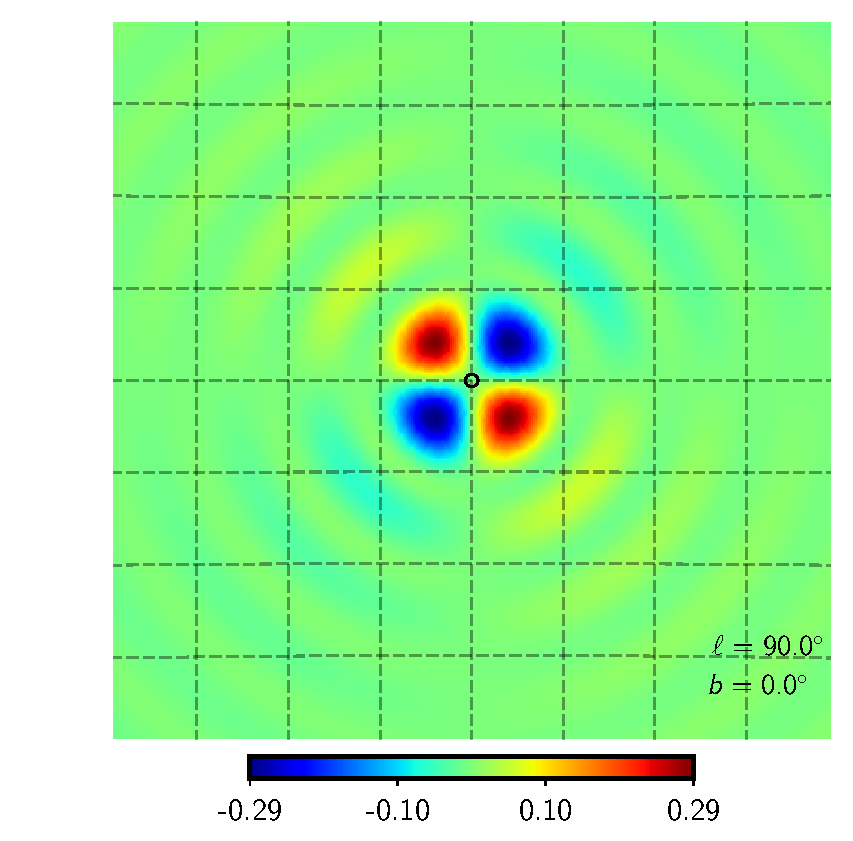
\includegraphics[width=0.16\columnwidth]{kernel/qu2eb_ker_i_lat0_lon90.pdf}}\hspace{-2mm}
\subfigure[$\mathcal{D}_r$]{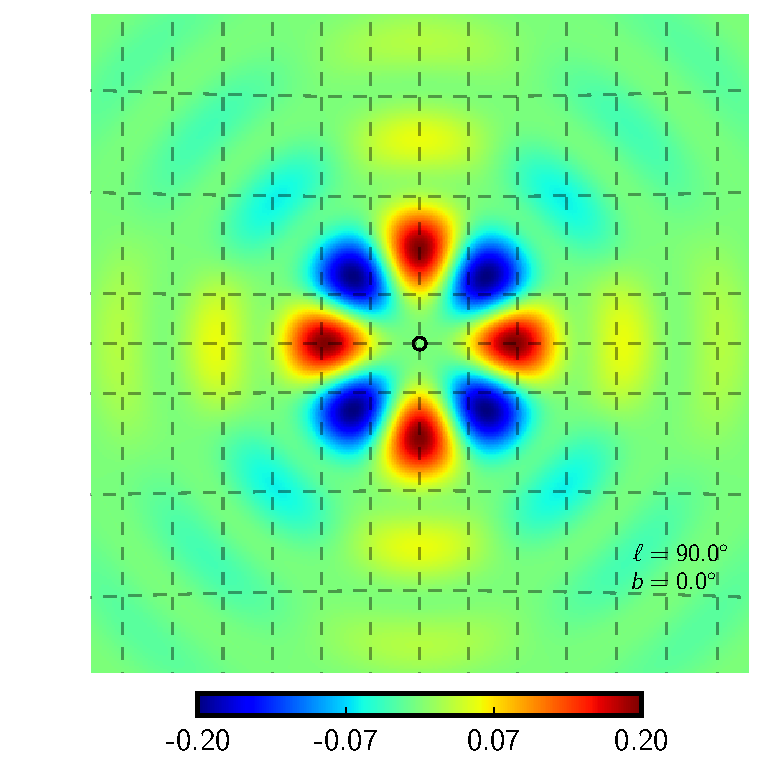
\includegraphics[width=0.16\columnwidth]{kernel/qu2ebqu_ker_r_lat0_lon90.pdf}}\hspace{-2mm}
\subfigure[$\mathcal{D}_i$]{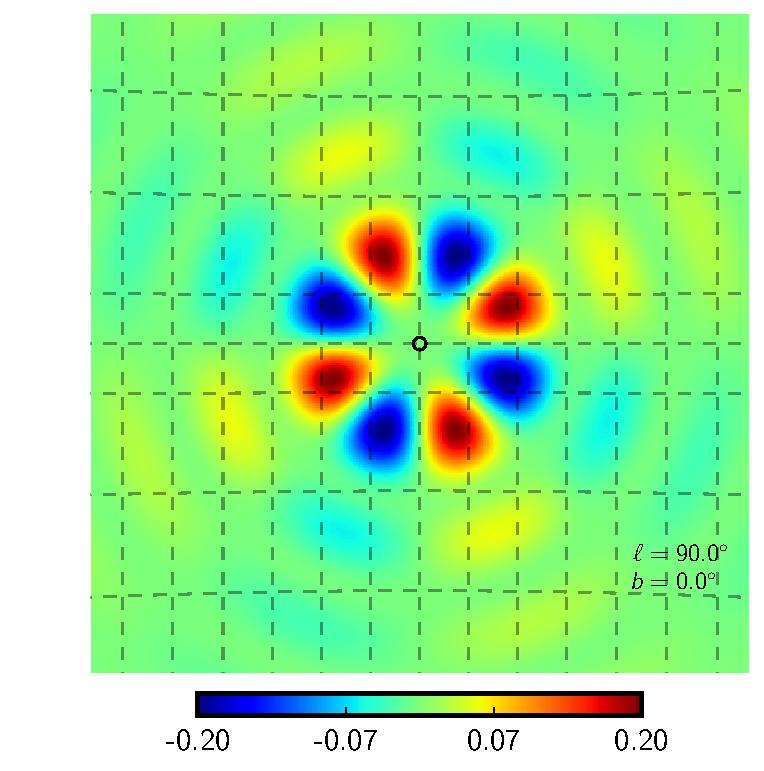
\includegraphics[width=0.16\columnwidth]{kernel/qu2ebqu_ker_i_lat0_lon90.pdf}}\hspace{-2mm}
\subfigure[$\mathcal{I}_r$]{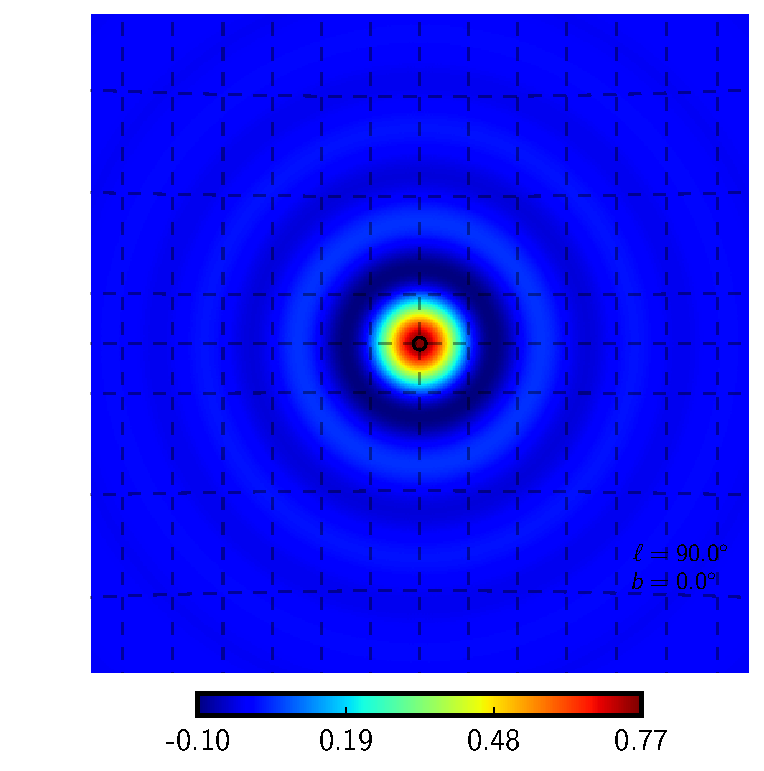
\includegraphics[width=0.16\columnwidth]{kernel/I_ker_r_lat0_lon90.pdf}}\hspace{-2mm}
\subfigure[$\mathcal{I}_i$]{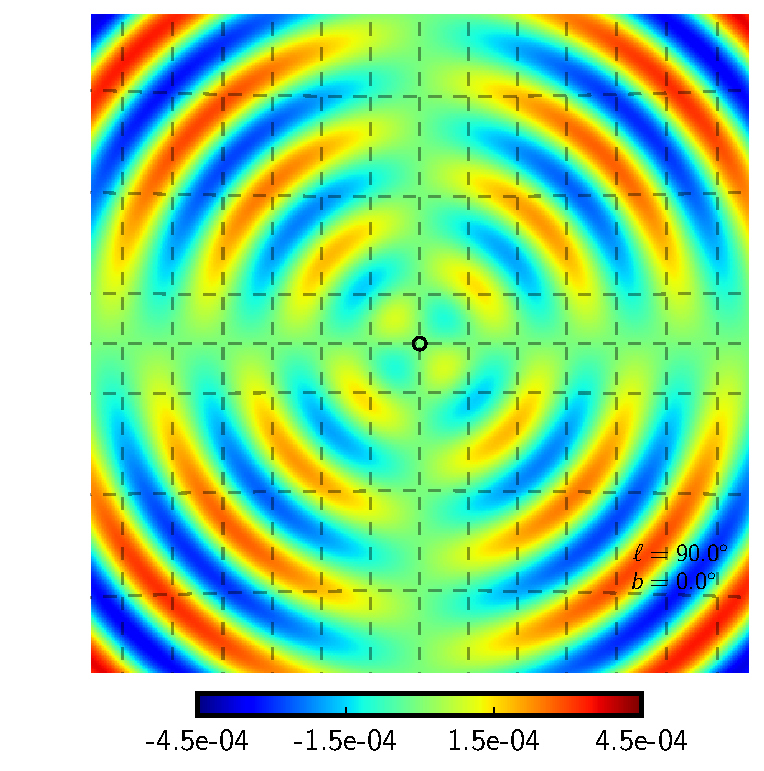
\includegraphics[width=0.16\columnwidth]{kernel/I_ker_i_lat0_lon90.pdf}}
\caption{This panel of figure depicts the various parts of the convolution kernel, discussed in \sec{sec:real_space_operators}. These kernels have been evaluated with the band limit: $\ell \in [2,192]$ but sampled at the Healpix resolution parameter NSIDE=2048 for visual appeal. The size of each panel is approximately $16^{\circ} \times 16^{\circ}$ and the grid lines are marked at 2 degree separations. The black circles denotes the position of the central pixel around which the convolution kernels have been evaluated while the black star marks the location of the north galactic pole. The four rows depict the kernels at different location on the sphere and the galactic coordinates of the central pixel are specified in each panel.}
%from top to bottom rows are as follows $[b,\ell] = [0^{\circ},0^{\circ}], [87^{\circ},0^{\circ}], [87^{\circ},30^{\circ}], [80^{\circ},30^{\circ}], [0^{\circ},90^{\circ}]$.}
\label{fig:vis_kernel}
 \end{figure}
%

\textit{Evaluating the local kernels: }\revisit{Let us consider the case when one of the coordinates coincides with the north pole $\hat{z}=(0,0)$ (this refers to the point $\theta_0 \rightarrow 0$ while moving along the longitude $\phi_0=0$). In this case the Euler angles in the $z-y1-z2$ convention are simply given by: $(\alpha,\beta,\gamma) =(\phi_i,\theta_i,0)$, where $(\theta_i,\phi_i)$ denote the coordinates of the location $\hat{n}_i$.} Since the Euler angle $\gamma=0$ when rotations are defined with respect to the pole, the respective kernels simplify to the following forms,
%
\begin{subequations}
\beqry 
\mathcal{M}(\hat{z},\hat{n}_i) &=&  \sum_{\ell} {{}_{0}}a_{\ell 2} \, {{}_{0}}Y_{\ell 2}(\hat{n}_i) \,;\\
\mathcal{I}(\hat{z},\hat{n}_i) &=& \sum_{\ell} {{}_{-2}}a_{\ell 2}\, {{}_{-2}}Y_{\ell 2}(\hat{n}_i) ~~\,;~~
\mathcal{D}(\hat{z},\hat{n}_i) =\sum_{\ell} {{}_{2}}a_{\ell 2} \, {{}_{2}}Y_{\ell 2}(\hat{n}_i) \,,
\eeqry
\end{subequations}
%
where ${}_{s}a_{\ell 2} = \sqrt{\frac{2 \ell+1}{ 4 \pi}} ~~\forall ~~ s \in [0,-2,+2]$.
The convolution kernels centered around any other location $\hat{n}_j = (\theta_j,\phi_j)$ are simply given by evaluating the respective spherical harmonic sums: $\sum_{\ell m} {}_{s}a_{\ell m}\,{}_{s}Y_{\ell m}(\hat{n}_i)$ using the rotated harmonic coefficients given by: ${}_s a_{\ell m} = D^{\ell}_{m 2}(\phi_j , \theta_j, 0) {{}_s}a_{\ell 2}$, where $D^{\ell}_{2 m}$ are the Wigner-D functions.
These rotation operations can be carried out using inbuilt Healpix routine \textit{rotate\_alm}, while the convolution kernels can be synthesized by evaluating the respective spherical harmonic sums using the \textit{alm2map} routine. 
\comment{Make parallels with instrument beam analysis here ? Or is it trivial since its obvious that all convolution problems can be cast in this form.}

We compute the local convolution kernels using the procedure described above. To given an intuition for how these kernels vary as a function of position of the central pixel we depict in \fig{fig:vis_kernel} the kernels at a few different locations.
For illustration these functions are sampled at a very high Healpix resolution parameter of NSIDE=2048. All the plots have been rotated such that the central location $\hat{n}_j$ marked by the black circle are in the centre of the figure. The horizontal and vertical lines that pass through the central black circle mark the local latitude and longitude respectively.

The real and imaginary part of the kernel $\mathcal{M}$ are identical irrespective of changes in the galactic latitude and longitude of the central pixel. Note that these functions are not distorted when a part of the domain overlaps with the poles, as can be seen in the first three rows of \fig{fig:vis_kernel}. Both these facts can be associated with the fact that this function does not depend on the Euler angle $\gamma$. From \eq{eq:qu2eb_convolution_explicit} and \eq{eq:eb2qu_convolution_explicit} it is clear that $\mathcal{M}_r$ and $\mathcal{M}_i$ can be interpreted in the following ways,
%\revisit{Recall that the angle $\gamma$ defines the rotation about the final z-axis which co-alligns the planar axes. Since the function $\mathcal{M}$ does not depend of this final orientation, it implies a rotational invariance of the fields constructed by convolving with this kernel.}
%
\begin{subequations}
\beqry
\bmat E= -\mathcal{M}_r \\ B =+\mathcal{M}_i  \emat  \leftarrow \bmat Q=\delta(\hat{n} - \hat{n}_j)\\ U=0 \emat ~~;~~ \bmat E= -\mathcal{M}_i \\ B = - \mathcal{M}_r  \emat  \leftarrow \bmat Q=0 \\ U=\delta(\hat{n} - \hat{n}_j) \emat \,,  \\
\bmat Q= -\mathcal{M}_r \\ U = -\mathcal{M}_i  \emat  \leftarrow \bmat E=\delta(\hat{n} - \hat{n}_j)\\ B=0 \emat ~~;~~ \bmat Q= +\mathcal{M}_i \\ U = - \mathcal{M}_r  \emat  \leftarrow \bmat E=0 \\ B=\delta(\hat{n} - \hat{n}_j) \emat \,.
\eeqry
\end{subequations}
%
The kernels $\mathcal{D}$ \& $\mathcal{I}$ vary significantly as a function of galactic latitude of the central pixel as seen in the last four columns of \fig{fig:vis_kernel}. These kernels show a two fold symmetry in the vicinity of the poles and this arises due to Euler angle $\gamma \approx 0$ here and therefore $e^{i2(\alpha \pm \gamma)} \approx e^{i2\alpha}$. Note that in this region, the azimuthal profile of the real and imaginary part of these kernels  is similar to $\mathcal{M}_r$ and $\mathcal{M}_i$ respectively.  This also explains why the imaginary part of the band limited delta function $\mathcal{I}$ contributes just as much as the real part in these regions. On moving to lower latitudes, $\mathcal{D}$ quickly transitions to having a four fold symmetry while $\mathcal{I}$ transitions to being dominated by the real part and behaves more like the conventional delta function. This transition can be most easily understood in the flat sky limit where $\gamma = -\alpha$ which leads to the resultant 4 fold symmetry seen for $\mathcal{D}$ owing to $e^{i2(\alpha - \gamma)} =e^{i4\alpha}$ and $\mathcal{I}$ being dominated by the real part owing to $e^{-i2(\alpha + \gamma)} =1 + i0$. Since the flat sky approximation has most validity in the proximity of the equator these limiting tendencies of the respective kernels are seen in the bottom row of \fig{fig:vis_kernel} which depict the kernels evaluated at the equator $b=0^{\circ}$. The middle two row depict the kernels evaluated at a latitudes of $b=87^{\circ}~\&~ 80^{\circ}$ and serve to indicate the rate of this transition. These kernels are invariant under changes in longitude of the central pixel, the latitude being held fixed, as one may have expected.

\subsection{Quantifying the non-locality of E \& B modes} \label{sec:radial_locality}
%
\begin{figure}[!hbt]
\centering
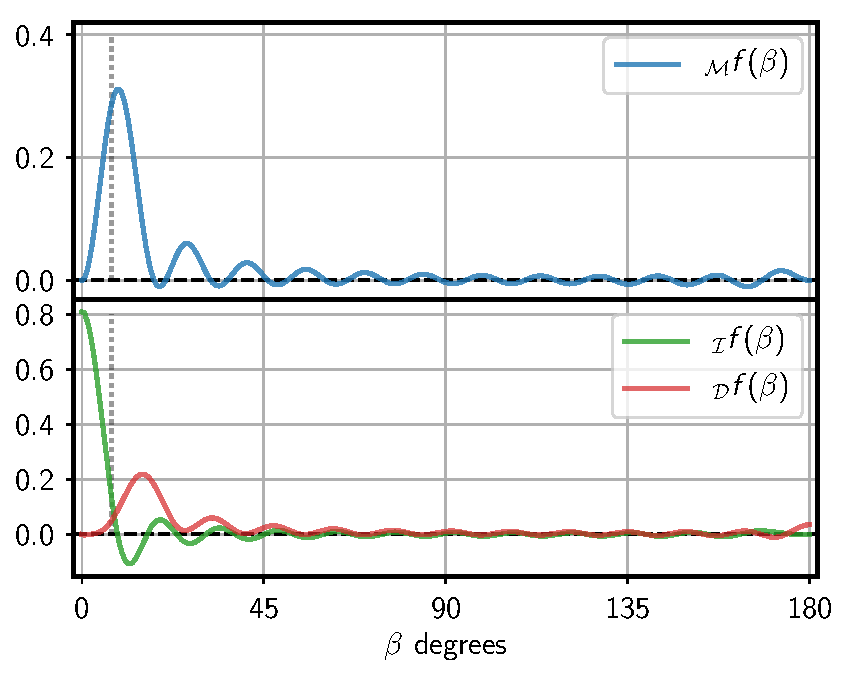
\includegraphics[width=0.8\columnwidth]{kernel/beta_kernel.pdf}
\caption{The figure depicts the radial part of the convolution kernels. These radial function have been evaluated with the band limit fixed at $\ell \in [2,24]$. The vertical dashed line marks the approximate Healpix pixel size of a NSIDE=8, which is the lowest resolution that allows access to $\ell_{\rm max}=24$.}
\label{fig:beta_kernel}
\end{figure}
%
\fig{fig:mixing_kernel} and the surrounding discussion provides a quantative understanding of the  azimuthal dependence of various kernels, however it is difficult to assess the radial nature of these kernels from these figures. The radial part determines the non-locality of the respective operators and encodes all the multipole dependence. We compute the radial kernels ${_{\mm}f}, {_{\md}f} ~\&~ {_{\mi}f} $ by evaluating the respective multipole sums in \eq{eq:rad_ker_queb} and \eq{eq:f2_rad_ker} in the band limit $\ell \in [2,192]$ and the resultant functions are depicted in \fig{fig:beta_kernel}. 

Recall that ${_{\mm}f}$ is the radial part of the kernel that translates the Stokes parameters $Q$ \& $U$ to scalars $E$ \& $B$ and vice versa. Note that ${_{\mm}f}$ has a vanishing contribution from the location of the central pixel ($\beta \rightarrow 0$) as seen in \fig{fig:beta_kernel} and one can show that that ${_{\mm}f(\beta=\pi)}=0$. The coordinate dependence of the Stokes parameters cannot be integrated out in the vicinity of the locations $\beta=0,\pi$ due to the fact that the azimuthal angles become ill defined here therefore this nature of ${_{\mm}f}$ is necessary to ensure that the derived fields behave as scalars. Similarly while deriving the Stoke field from the scalars $E$ \& $B$ this nature of ${_{\mm}f}$ is necessary to ensure that the necessary coordinate dependencies are integrated in. ${_{\md}f}$ shows a similar behaviour, it has a vanishing contribution in the vicinity of the central pixel and dominantly contributes in regions which are approximately at least 1 pixel distance away from the central pixel as seen in \fig{fig:beta_kernel}. ${_{\mi}f}$ is the radial part of the band limited delta function $\mi$ and expectedly contributes the most at the location of the central pixel. 


\noindent \textit{The band limit dependence:} It is clear from previous discussions that the scalar field $E$ \& $B$ constructed at a location depends on the Stokes field in the surrounding regions. We further quantify this non-locality by studying the radial extent of the kernels and its dependence on the maximum multipole accessible for analysis. To carry out this study we evaluate the radial functions for different values of $\ell_{\rm max}$, while keeping the lowest multipole fixed at $\ell_{\rm min}=2$. 
%
\begin{figure}[t]
\centering
\subfigure{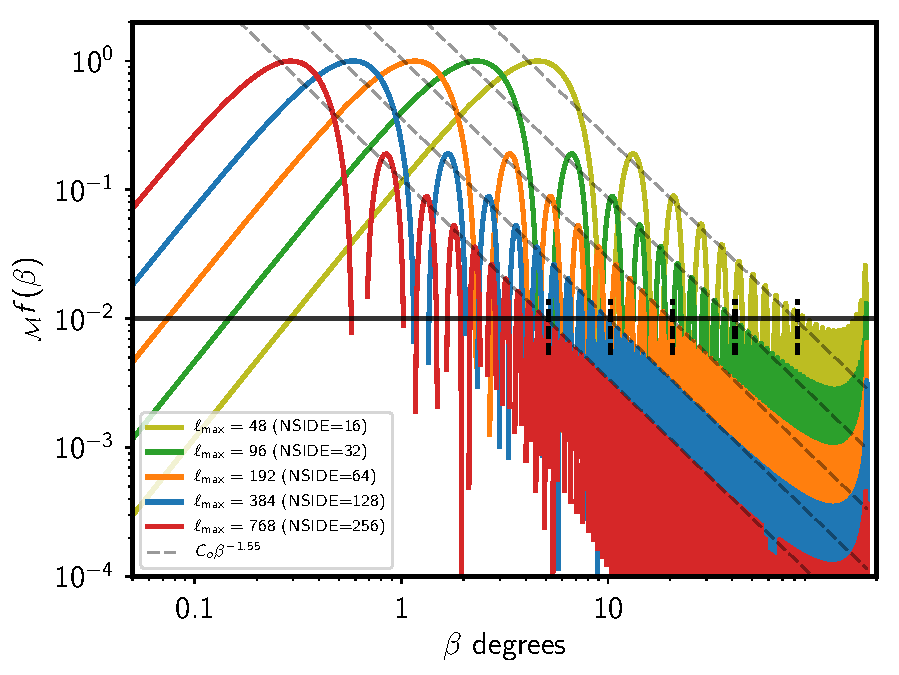
\includegraphics[width=0.96\columnwidth]{kernel/f_rad_ker_fn_of_ellmax.pdf}}
\subfigure{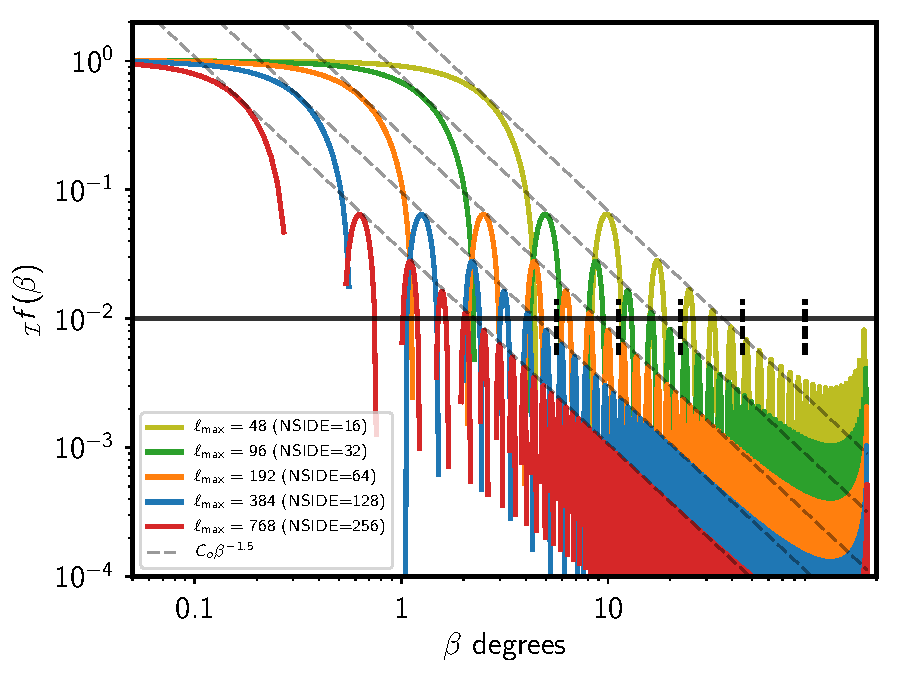
\includegraphics[width=0.48\columnwidth]{kernel/fm2_rad_ker_fn_of_ellmax.pdf}}
\subfigure{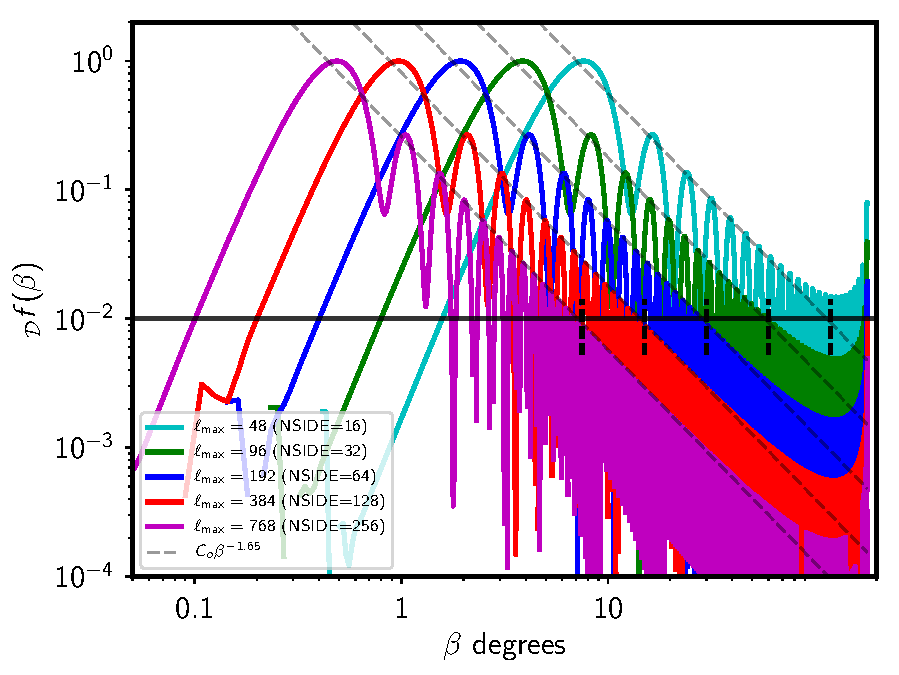
\includegraphics[width=0.48\columnwidth]{kernel/fp2_rad_ker_fn_of_ellmax.pdf}}
\caption{The top panel depicts the radial function  ${_{\mm}f}(\beta,\ell_{\rm min},\ell_{\rm max})$ while the bottom left and right panels show the radial functions ${}_{\mi}f(\beta,\ell_{\rm min},\ell_{\rm max}) ~\&~ {}_{\md}f(\beta,\ell_{\rm min},\ell_{\rm max})$ respectively, for fixed $\ell_{\rm min}=2$ and different $\ell_{\rm max}$ as indicated by their legends. All the curves have been normalized such that the maximum of the curve is set to unity. The horizontal solid black line marks the location where the amplitude of the kernel falls below 1\% of its maximum. The slanted dashed black lines indicate a power law fit (by eye) to the envelope of the radial functions. While the envelopes for function ${_{\mm}f}(\beta)~\&~ {}_{\mi}f(\beta)$ are fit well by the power law $\propto \beta^{-1.5}$, the envelope for the function ${}_{\md}f(\beta)$ is seen to have a slightly steeper slope $\propto \beta^{-1.65}$.}
\label{fig:rad_ker_decay}
\end{figure}
%
The resultant set of radial function are depicted in \fig{fig:rad_ker_decay}, where all the function have been normalized such that their global maxima is set to unity. We note that on increasing $\ell_{\rm max}$ the radial kernels shift left, attaining their global maxima at progressively small angular distance from the central pixel. The amplitude of these radial function scales up as $\propto \ell_{\rm max}^2$. At intermediate values of $\beta$, the envelope of the radial functions is fit well by a power law $ \propto \beta^{-n}$, the details of this fit can be seen in \fig{fig:rad_ker_decay}.
We observe that the radial functions computed by evaluating the multipole sums to different maximum multipoles are self similar and follow an interesting telescoping and scaling property, $${}_rf(\beta,2,\ell_{\rm max}) \approx \Big[\frac{\ell_{\rm max}}{\ell'_{\rm max}}\Big]^2{}_rf(\beta'=\frac{\ell_{\rm max}}{\ell'_{\rm max}} \beta ,2,\ell'_{\rm max}) \,,$$ where ${}_rf$ denotes all the different radial functions. 
%We can understand the shifting left of the radial kernels on increasing the maximum multipole using this property. Lets say the function ${}_rf(\beta, \ell'_{\rm max})$ transition to being monotonously below some fraction of the global maxima at an angular distance of $\beta_0$.  The function ${}_rf(\beta', \ell_{\rm max})$, given $\ell_{\rm max} > \ell'_{\rm max}$, reaches the same transition point $\beta'=\beta_0$ at a smaller value of $\beta$ owing to the fact that $\ell_{\rm max}/\ell'_{\rm max}$ is greater than unity. The amplitude scaling of the functions is irrelevant since the transition point is always described in terms of the fraction of the global maxima of the function.

It is useful to define a characteristic radius of the region from which the scalar fields evaluated at a point get most of their contribution from.  Since the primarily interest is in the non-locality of the scalar modes $E$ \& $B$ we define the abscissa at which the function ${_{\mm}f}(\beta,\ell_{\rm min}=2,\ell_{\rm max})$ transits to being monotonously below 1\% of the maxima of the function as the non-locality parameter: $\beta_{o}$.  For $\ell_{\rm max}=24$, the maximum multipole accessible on a Nside=8 Healpix map, the non-locality parameter $\beta_0=180^{\circ}$ as the radial function never falls monotonously below 1\% of its global maxima. Using this fact and the self similar property of the radial functions, we define the following empirical relation: $\beta_o= {\rm min}(180,180 \frac{24}{\ell_{\rm max}})$, as a means of estimating the non-locality parameter given the maximum multipole $\ell_{\rm max}$ accessible for analysis.